\documentclass[10pt]{article} 

\makeatletter
\renewcommand\section{\@startsection{section}{1}{\z@}%
                                  {-3.5ex \@plus -1ex \@minus -.2ex}%
                                  {2.3ex \@plus.2ex}%
                                  {\normalfont\large\bfseries}}
\makeatother

\addtolength{\oddsidemargin}{-.875in}
\addtolength{\evensidemargin}{-.875in}
\addtolength{\textwidth}{1.75in}
\addtolength{\topmargin}{-.875in}
\addtolength{\textheight}{1.75in}

\usepackage{titlesec, graphicx, titling, fancyhdr}
\setlength{\droptitle}{-6em}
\posttitle{\par\end{center}\vspace{-4.8em}}

\pagestyle{fancyplain}
\renewcommand{\headrulewidth}{0pt}
\newcommand{\advsection}{\addtocounter{section}{1} }

\begin{document}

\lhead{Frederick Robinson}
\rhead{Quiz 2}

%\section{Let $$f(x) = \sqrt{\frac{(x^2 -1)^3}{(x^2 +2)^5}}.$$ Find $f'(x)$. Simplify your answer.}
\advsection

\section{A function $y=f(x)$ is defined implicity by the equation $(x+y^2)^3 - (x y )^3 - 7 =0 $. Show that the point $(1,1)$ lies on the graph of $f(x)$ and then find the equation of the \emph{normal} line to the graph of $f(x)$ at the point $(1,1)$.}

First plug in $x=1, y=1$ to verify that the point lies on the graph:
\[(1 + 1^2)^3 - 1^3 - 7 =0.\]

To find the equation of the normal, first find the slope of the tangent by implicit differentiation:
\[(x+y^2)^3 - (x y )^3 - 7 =0  \Rightarrow 3(x+y^2)^2 (dx + 2 y dy)=3(x y)^2 (xdy + y dx) \]
so at $(1,1)$ we have 
\[3(1+1^2)^2 (dx + 2 dy)=3(1\cdot 1)^2 (dy + dx) \Rightarrow 12(dx + 2 dy) = 3 (dy + dx) \Rightarrow \frac{dy}{dx} = - 3/7\]

Therefore, the slope of the \emph{normal} is $-1/ (-3/7) = 7/3$. The equation is therefore given by 
\[y - 1 = 7/3(x - 1) \iff y = \frac{7}{3} x -\frac{4}{3} \]

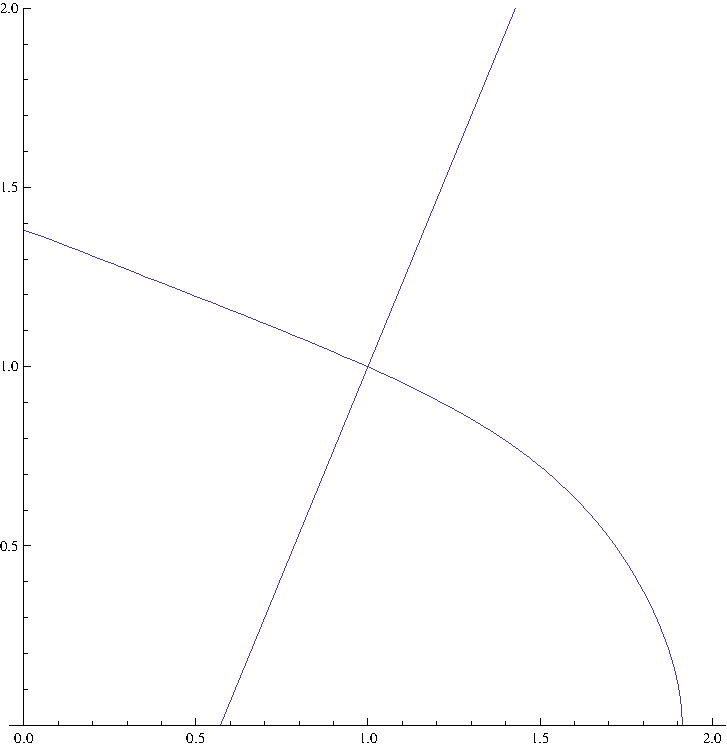
\includegraphics{quiz2plot1}

%\section{An inverted conical tank has height $h = 8$ft and radius $r =4$ft. If water is pumped \emph{into} the tank at a  rate of 1 cubic ft/sec then how fast is the \emph{radius} increasing when the water level is 3 feet?} 

\end{document}
